\section{一些图形模板}

\subsection{流程图}
流程图如\ref{do_asy}:
\begin{figure}[H]%位置选项
\centering
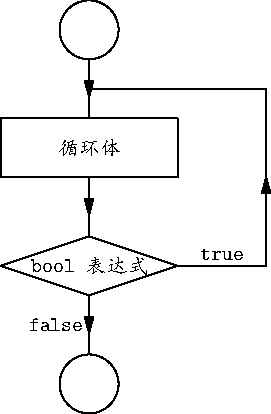
\includegraphics[width=6cm]{do}
\caption{流程图} \label{do_asy}
\end{figure}

代码如下所示:

  \lstinputlisting{figures/do.asy}






\subsection{状态机}
首先将 simplenode.asy 放至 Asymptote 的安装文件夹,再执行 automata 的 asy 文件。
\begin{figure}[H]%位置选项
\centering
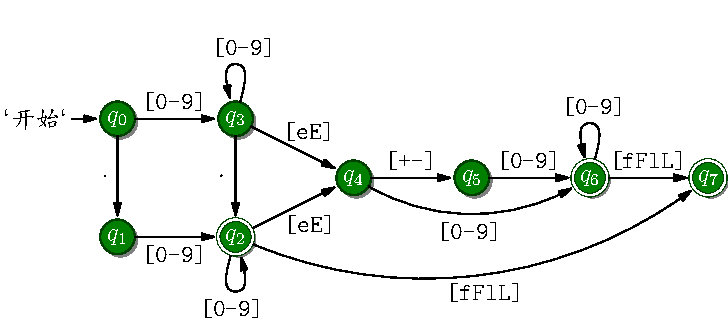
\includegraphics[width=14cm]{body/asycode/automata}
\caption{状态机} \label{automata}
\end{figure}

\subsubsection{源代码}


代码如下所示。\label{code_automata}
  \lstinputlisting{body/asycode/automata.asy}

\subsection{时序图}
\begin{figure}[H]%位置选项
\centering
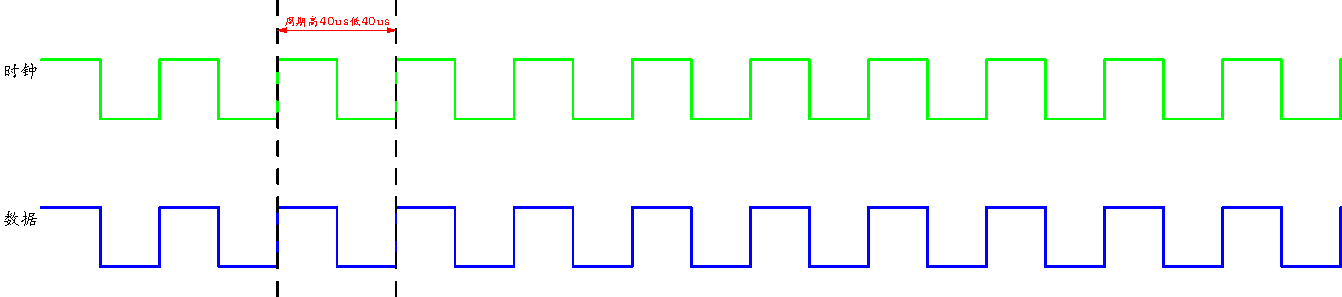
\includegraphics[width=14cm]{body/asycode/wave}
\caption{时序图} \label{wave}
\end{figure}
代码如下所示
\tiny
  \lstinputlisting{body/asycode/wave.asy}
  \normalsize 